%%This is a very basic article template.
%%There is just one section and two subsections.
% \documentclass{article}
%\documentclass[phd,ilcc,twoside]{infthesis}
\documentclass[bsc,logo, abbrevs]{infthesis}
\course{Institute for Language, Cognition and Computation}
\project{\textbf{Supervisor}: Prof. XYZ}

% This package is for times font
\usepackage{times}

% This package is for Informatics thesis style
\usepackage{eushield}

% This package is for your references
\usepackage[numbers]{natbib}

% This package is for figures
\usepackage{graphicx}

% This package is for urls
\usepackage{url}

% For symbols and equations 
\usepackage{latexsym}
\usepackage{amsmath}
\usepackage{acronym}

%% Information about the title, etc.
\title{Personalized Air Quality Visualization and Tracking}
\author{Alberto Vazquez Martinez}

%% Specify the abstract here.
%\abstract{%
%
%Abstract for my Report
%}

\begin{document}

%% First, the preliminary pages
\begin{preliminary}

\maketitle

%% Create the table of contents
\standarddeclaration
\dedication{To my mummy.}
\tableofcontents
\listoffigures
\listoftables
\begin{accron}\begin{acronym}[MPC] % Give the longest label here so that the list is nicely aligned
\acro{MPC}{model predictive control}
\acro{TLA}{Three Letter Acronym}
\acro{COMEAP}{Committee on the Medical Effects of Air Pollutants}
\acro{DEFRA}{Department for Environment Food and Rural Affairs}
\acro{NO2}{Nitrogen Dioxide}
\acro{O}[O\textsubscript{3}]{Ozone}
\acro{SO}[SO\textsubscript{2}]{Sulphur Dioxide}
\acro{NO}[NO\textsubscript{x}]{Nitrogen Oxides}
\acro{PM}{Particle Matter}
\acro{PM}[PM\textsubscript{10}]{Particle Matter 10 micrometer}
\acro{PM}[PM\textsubscript{2.5}]{Particle Matter 2.5 micrometer}
\acro{IaaS}{Infrastructure as a service}
\acro{UI}{User Interface}
\acro{API}{Application Programming Interfaces}
\acro{CMEAP}{Committee on the medical effects of air pollutants}

\end{acronym}\end{accron}

\end{preliminary}

\chapter{Introduction}
Breathing fresh air is a right that everyone should have.
In recent years air quality has taken on an increasingly important role in people's lives as well as government institutions which are increasingly aware of the hazards of air pollution. In Scotland alone there are in total 32 ``pollution zones'' that are considered to breach European safety standards \cite{Foe-scotland.org.uk} \cite{OKScotland2015}. The negative impact of poor air on our health, diminishing our life quality and causing cardiovascular and respiratory diseases is of greater concern. As such, new air quality monitoring sensors are being developed and deployed. Some of them are in fixed locations, whilst others are carried around. Data is becoming more available and fine-grained providing a further capability to enable educated decisions.

Through this new outsourced data, it is possible to tackle the pollution problem by taking a  more personalised approach as ``everyone has different needs and lifestyles that expose them differently to pollution'' \cite{Vazquez2016}. Different population groups are more vulnerable than others. For example, children are more affected than adults because their lungs are still developing. Furthermore, people with respiratory diseases suffer from aggravated symptoms because their airways get irritated with spikes in air pollution. The way data is presented and disseminated to the public is crucial part of the solution. Therefore, digitally enabled visualisation is an excellent tool that unleashes the full potential of data; as new technologies are available to extract, filter, display and animate it evoking the interest and attention of the people while providing unique experiences and mechanisms to improve their lives.

\iffalse
The effects of air pollution on human health are still complex to understand and there is much research ongoing on the combination short and long term effects upon a person's health. 
\fi
\section{Aims and Objectives}
The first aim of this project is to review current approaches to air quality data dissemination and visualisation. Furthermore, this project examines the current needs of pollution-sensitive and non-sensitive users in relation to a new air-quality data dissemination tool to accomplish the main goal: to develop and implement a mobile application to visualise air quality data in a useful and understandable way.

Another important objective is to take on a more user-centred approach whilst achieving this main goal, by bearing in mind the users as co-designers and stakeholders throughout three different design iterations of the product for the creation of a final prototype that reflects more accurately the user needs and thoughts.

\iffalse
DATA -> APP -> USEFUL -> PERSONAL -> DECISION SUPPORT -> DESIGNED BY PEOPLE
\fi
\input{1-introduction/3-Challenges}
\section{Dissertation Outline}
This dissertation is structured as follows: 
 
\bigskip
 Chapter 2: Background
\bigskip

This chapter discusses relevant background topics key to understanding the dissertation. It explains the project's importance in the context of the pollution problem, including definitions to follow the basic air quality dissemination terms and related health issues. Past approaches for visualising are also discussed and critically evaluated, as well as explaining in detail what is meant by data visualisation and how to achieve it from a decision support perspective.
 
\bigskip
 Chapter 3: Methodology
\bigskip
  
This chapter describes the methodology and processes that have been used throughout the project. It describes how the development was addressed not only from a human-computer interaction perspective but as well from a software engineering perspective. 
  
\bigskip  
 Chapter 4: Analysis and Design
\bigskip

The analysis and design of the system are  both addressed in this chapter. A detailed analysis of the current needs of a new air quality application are presented, as well as explaining the design and infrastructure choices made for achieving the project goal in a way all stakeholders are considered. The first application prototype is presented.
 
\bigskip
Chapter 5: Implementation
\bigskip

This chapter describes how the required infrastructure and software components were set-up to proceed with the implementation of the final two prototypes, as well as the transitional choices that resulted from the user-centred development approach.

\bigskip
 Chapter 6: Evaluation
\bigskip

The final technical and user evaluations are presented in this chapter by describing how well the defined requirements in Chapter 4 were met with quantitative and qualitative methods.

\bigskip
 Chapter 7: Conclusion
\bigskip

This chapter looks at the aims of the dissertation from an integrative perspective highlighting what has been accomplished so far and giving recommendations for future research.
\chapter{Background}
\section{Air Quality}
\subsection{Air pollution and its health effects}
Air pollution can be defined as a group of chemicals present in the atmosphere that are harmful to humans, animals or vegetation. It is mainly caused by human activities, such as transport, industry, or agriculture. But it can also be influenced by other natural sources. Understanding air pollution is important because many health consequences result from high pollution levels. 
\begin{figure}[h]
  \centering
  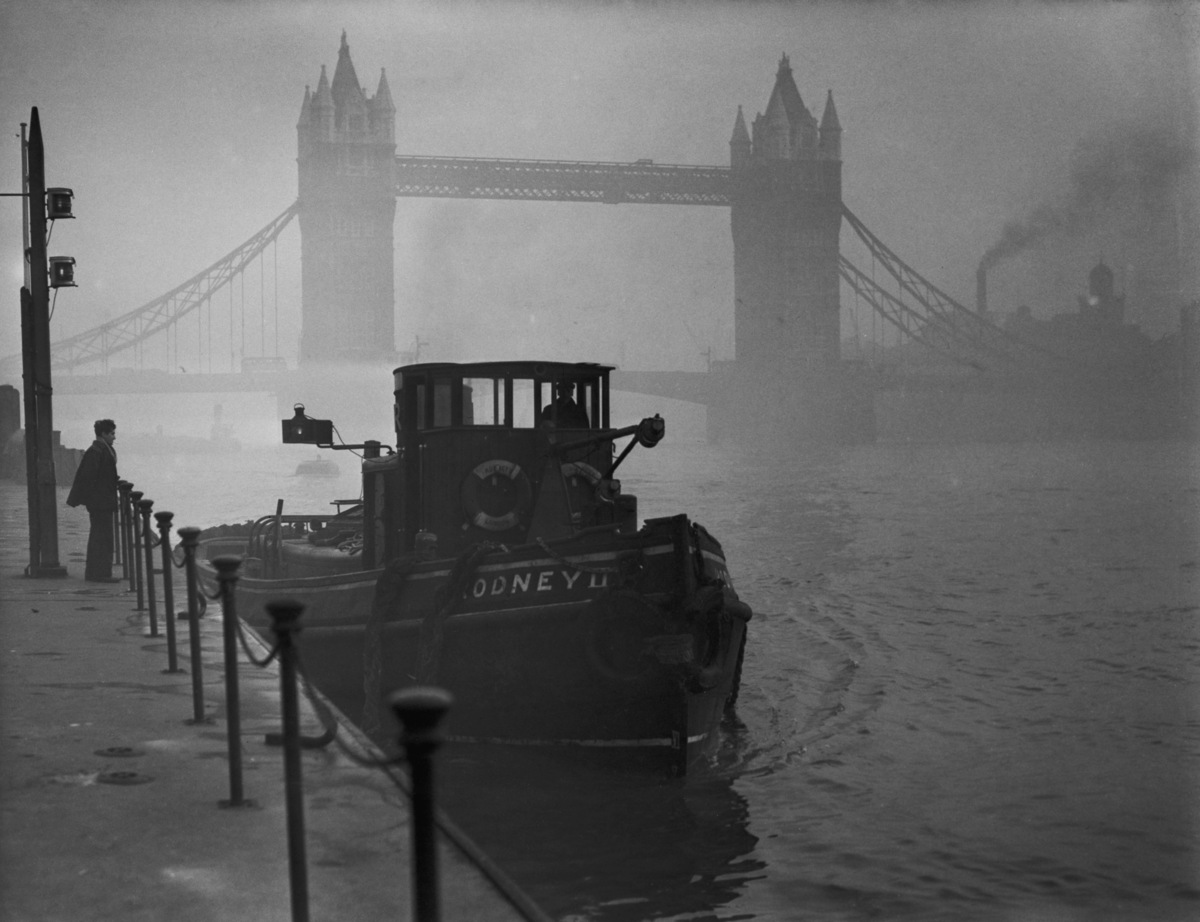
\includegraphics[scale=.8]{images/great_smog.jpg}
  \caption[Great smog of 1952]{Great smog of 1952 \cite{ElliotWagland2013}}
  \label{fig:interaction_design}
\end{figure}

One historic event which caused huge consequences is known as the great smog of 1952. Thousands of people died in Greater London due to exposure over several days to a highly contaminated atmosphere, and many others became ill or experienced retarded symptoms \cite{Bell2008}. The fog originated from coal burning, vehicle exhaust and other atmospheric factors. Although many human activities introducing pollution have changed since then, it became evident the immediate and retarded health impact of pollution. 

Pollution particles can be categorised into gaseous pollutants, persistent organic pollutants, heavy metals and particulate matter. They vary in their chemical composition, emission sources and impact on health. 

Gaseous pollutants are sulphur dioxide (\SOTWO), nitrogen oxides (\NOX), carbon monoxide (CO), ozone (\OTHREE) and volatile organic compounds (VOCs). The principal source of gaseous pollutants is combustion of fossil fuels and diesel emission from vehicles. Nitrogen oxides (\NOX) is a general term that includes nitric oxide (NO) and nitrogen oxide \NOTWO. Gaseous pollutants can affect our health by inflaming the airways and lungs, and in the long term, affect the function of the lungs \cite{AirQualityExpertGroup2004} \cite{WHO2003}.

Particulate matter (PM) is a mixture of solid and liquid particles (such as sulphate, nitrates, ammonia, sodium chloride, black carbon, mineral dust and water). PM are categorised according to their diameter size measured in microns (\SI{}{\micro\metre}, one millionth of a metre). Particles smaller than 10 microns (\PMTEN) are known as coarse particles, smaller particles with a size of up to 2.5 and 1 microns (\PMTWO and \PMONE) are known as fine and ultra-fine particles respectively. They are differentiated in sizes because it dictates their aerodynamic properties, that is, how they are transported into the air, as well as how far they can get into the respiratory system. According to the World Health Organization, PM is the most harmful pollutant because it can pass through the nose and throat and enter the lungs, there is also evidence that it is associated with risk of cardiovascular disease \cite{Polichetti2009}. 

Air quality is also affected by pollution mixture in further complex chemical structures and by temperature and humidity conditions. \NOTWO, PM and O\textsubscript{3}  pollutants get transformed by atmospheric processes making it hard to evaluate their individual impact. As an example, ground level ozone is produced when sunlight interacts with \NOTWO and volatile organic compounds. Furthermore, \NOTWO and other nitrogen oxides also contribute to PM generation, making \NOX a particularly concerning pollutant.

\subsection{Air quality data dissemination}
Openly published air quality data aimed to have informed and aware citizens that could take part into more sustainable and environmental choices. \quotes{Yet, what was lacking (and it still is), is a model for effective communicating of environmental information to the public} \cite{Thinh2007}. Terms like assessment, limit values, target values and concentration, among others, are commonly used by air quality data publishers to describe the current or forecasted quality status; however, there is not general agreement on how air quality information should be disseminated to the general public in a way it is understood immediately and intuitively. 

In general it is complex to categorise and establish measures for the different components of air pollution due their heterogeneous nature and the chemical reactions that occur between them. Measurement methods and units vary from institution to institution and regulation standards can be specific for each country, which may give rise to ambiguity. Furthermore, much of the available data is represented in a tabular format, including various information for individual pollutants, as exemplified in table \ref{tab:pollution_tabular_data}. This table was extracted from the  Department for Environment Food and Rural Affairs (DEFRA) website \cite{DepartmentforEnvironmenta}, and shows measures related to the air quality from a sensing station located in Deaconess Garden in the south of Edinburgh. At first sight it table arises some questions for the novice on air-quality trying to crack the data. Firstly, the pollution codes such as PM2.5, PM10, NO2, NOX as NO2 and their subtle differences should be understood. Secondly, some measurement units are tagged with the monitoring method used to extract the information, like the TEOM FDMS \footnote{Which indicates that the sensing methods were Tapered Element Oscillating Microbalance and Filter Dynamics Measurement System \cite{Quality2005}} tag. And lastly, it is hard to know which measurements are of more interest given a person's particular circumstances. As stated by Brimblecombe and Schuepbach \cite{P.Brimblecombe2008}, \quotes{many people complain that the information is unintelligible, while some have even seen it as an attempt of government to blind the public with science}.  It is clearly difficult to understand the meaning of the terms and values that are used to represent air quality data to the general public. 

\begin{table}[ht]
\centering
\begin{adjustbox}{width=1.2\textwidth,center=\textwidth}
\begin{tabular}{rlrrrrrrr}
  \hline
 Pollutant & Date & Time & Measurement & Unit & Period & Comment  \\ \hline
    Ozone (O3) & 20/07/2016 & 07:00 & 63.06412 & µg/m3 & Hourly & - \\
    Nitric oxide (NO) & 20/07/2016 & 07:00 & 2.61933 & µg/m3 & Hourly & - \\
    Nitrogen dioxide (NO2) & 20/07/2016 & 07:00 & 27.34875 & µg/m3 & Hourly & - \\
    Nitrogen oxides as nitrogen dioxide (NOXasNO2) & 20/07/2016 & 07:00 & 31.36500 & µg/m3 & Hourly & - \\
	Sulphur dioxide (SO2) & 20/07/2016 & 07:00 & 14.63495 & µg/m3 & Hourly & - \\
	Carbon monoxide (CO) & 20/07/2016 & 07:00 & 0.081494 & mg/m3 & Hourly & - \\
	PM10 particulate matter (Hourly measured) (PM10) & 18/07/2016 & 15:00 & 10.900 & µg/m3 (TEOM FDMS) & Hourly & - No current data. \\
	Non-volatile PM10 (Hourly measured) (Non-volatile PM10) & 19/07/2016 & 07:00 & 26.700 & µg/m3 (TEOM FDMS) & Hourly & - No current data. \\
	Volatile PM10 (Hourly measured) (Volatile PM10) & 19/07/2016 & 07:00 & 5.500 & µg/m3 (TEOM FDMS) & Hourly & - No current data. \\
	PM2.5 particulate matter (Hourly measured) (PM2.5) & 18/07/2016 & 15:00 & 4.300 & µg/m3 (TEOM FDMS) & Hourly & - No current data. \\
	Non-volatile PM2.5 (Hourly measured) (Non-volatile PM2.5) & 19/07/2016 & 07:00 & 16.300 & µg/m3 (TEOM FDMS) & Hourly & - No current data. \\
	Volatile PM2.5 (Hourly measured) (Volatile PM2.5) & 19/07/2016 & 07:00 & 5.000 & µg/m3 (TEOM FDMS) & Hourly & - No current data. \\
	Modelled Wind Direction (Dir) & 19/07/2016 & 24:00 & 50.6 & \degree & Hourly & - No current data. \\
	Modelled Wind Speed (Speed) & 19/07/2016 & 24:00 & 6.2 & m/s & Hourly & - No current data. \\
	Modelled Temperature (Temp) & 19/07/2016 & 24:00 & 14.6 & °C & Hourly & - No current data. \\
	PM10 Ambient Temperature (AT10) & 19/07/2016 & 07:00 & 19.4 & °C & Hourly & - No current data. \\
	PM10 Ambient pressure measured (AP10) & 19/07/2016 & 07:00 & 989.0 & mb & Hourly & - No current data. \\
	PM2.5 Ambient Temperature (AT25 ) & 19/07/2016 & 07:00 & 17.5 & °C & Hourly & - No current data. \\
	PM2.5 Ambient Preasure (AP25) & 19/07/2016 & 07:00 & 988.0 & mb & Hourly & - No current data. \\
   \hline
\end{tabular}
\end{adjustbox}
\caption{Air quality tabular data representation. \cite{DepartmentforEnvironment}}
\label{tab:pollution_tabular_data}
\end{table} 

\subsection{The COMEAP air quality index and health advice}
In order to understand the correlation between air quality data and its effects on human health, the Committee on the Medical Effects of Air Pollutants (COMEAP) developed the air quality index based on health evidence. It is used to communicate real-time air quality levels and their short-term health effects for five selected harmful pollutants: particulate matter (\PMTEN and \PMTWO), ozone (\OTHREE), sulphur dioxide (\SOTWO), and nitrogen dioxide (\NOTWO) as shown in Figure \ref{fig:air_quality_index}. The index employs a colour scale and a number index to inform about how high are the concentrations of each specific pollutant. Four bands are employed: Low, Moderate, High and Very High. 

\begin{figure}[H]
\begin{adjustbox}{width=1\textwidth,center=\textwidth}
  \centering
  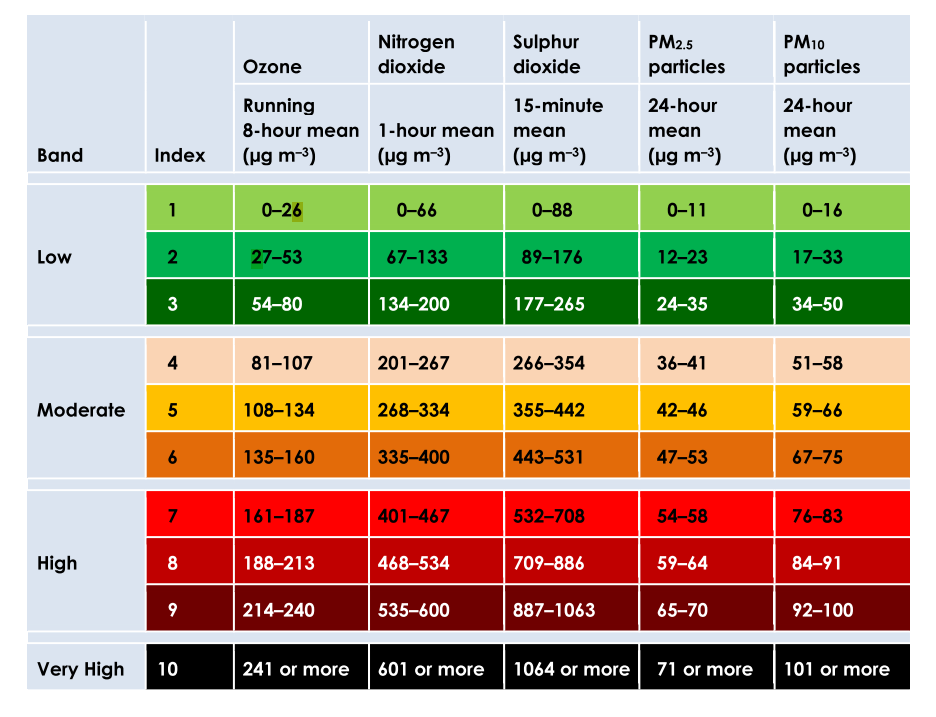
\includegraphics[scale=.8]{images/air_quality_index.png}
\end{adjustbox}
  \caption[The COMEAP air quality index]{The COMEAP air quality index \cite{HealthProtectionAgencyfortheCommitteeontheMedicalEffectsofAirPollutants2011}}
  \label{fig:air_quality_index}
\end{figure}

There is substantial evidence that the elderly, children, and persons that suffer from chronic diseases such as asthma are in greater danger of suffering symptoms and health consequences from lower pollution concentrations than the general public \cite{Koenig1999} \cite{Kampa2008} \cite{Zones2010} . The COMEAP includes such population in their Air Quality Index to give them the opportunity to modify their behaviour and reduce the severity of their symptoms. Furthermore, the air quality index is accompanied by a health advice (Figure \ref{fig:air_quality_health_advice}) which provides specific health messages targeting both population groups, sensitive and non-sensitive providing information about the actions that should be taken to avoid symptoms and health effects.

\begin{figure}[H]
\begin{adjustbox}{width=1\textwidth,center=\textwidth}
  \centering
  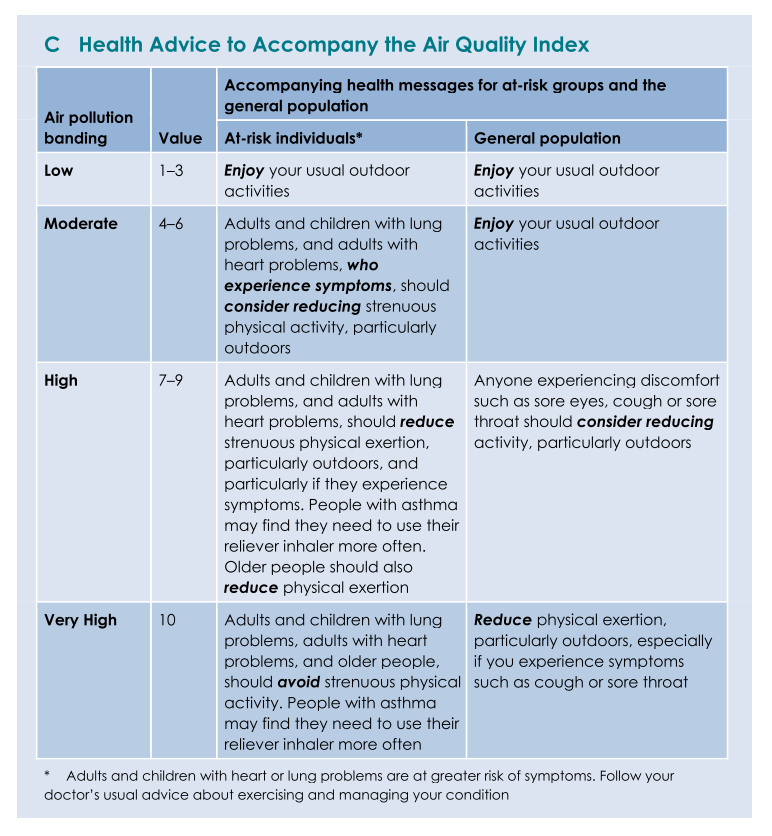
\includegraphics[scale=.8]{images/air_quality_health_advice.png}
\end{adjustbox}
  \caption[Air quality health advice]{Air quality health advice \cite{HealthProtectionAgencyfortheCommitteeontheMedicalEffectsofAirPollutants2011}}
  \label{fig:air_quality_health_advice}
\end{figure}


\subsection{Air quality sensors}

\begin{itemize}

\item Fixed sensors: 

Fixed sensors are installed and maintained by the UK government and local authorities in Scotland. There are of two kinds, automatic sensors from the Automatic Urban and Rural Network (AURN)\footnote{\url{https://uk-air.defra.gov.uk/networks/network-info?view=aurn}}, and non automatic sensors maintained by local Scottish councils. 

	\begin{itemize}
    
    \item Automatic sensors: They produce hourly concentrations and data is sent automatically over the network. They purpose is to check that EU and other regulatory standards are being met as well as informing the public about air quality. These sensors monitor a wide range of pollutants (\NOX, \SOTWO, CO\textsubscript{2}, O\textsubscript{3}, \PMTWO and \PMTEN) which are later collected and processed by Ricardo Energy and Environment \footnote{\url{http://ee.ricardo.com}} and exposed through HTML webpages at the Scottish Air Quality website\footnote{\url{http://www.scottishairquality.co.uk/}} or CSV files provided on demand. 
	\item Non automatic sensors: 
    
    \end{itemize}

\item Portable sensors:

\item Participatory sensors:

Some projects such as CitiSense \cite{Nikzad2012} include users as 'human sensors' by reading their perceptions towards air quality in certain locations. This method aims to get more fine-grained information about air quality and engage the citizens in the pollution problem and its solution. 

\end{itemize}




\section{Air Pollution Health effects}

 The health effects of NO\textsubscript{x} are irritating the lungs and increasing susceptibility to respiratory infections like influenza[].
 According to the World Health Organization, PM is the most harmful pollutant because it can pass through the nose and throat and enter the lungs. PM 
 
Exposure to PM is associated with risk of cardiovascular disease \cite{Polichetti2009}


\section{Decision Support Systems}
\section{Air Quality Applications}
\section{Air Quality Data}
\input{2-background/6-Data-Visualization}
\chapter{Methodology}
In order to accomplish the project aim, it is imperative to select a framework which allows a user inclusive development process as well as a flexible and iterative workflow. The project followed an interaction design model and an agile development methodology. The following sections will give a brief outline of these methods, as well as describe how they have been used throughout the project.
\section{Interaction Design Process}
Interaction design can be briefly defined as "designing interactive products to support people in their everyday working lives" \cite{Sharp2011}. To develop a useful product an understanding of what is needed must be established before and during the development process. This brings new challenges and questions, such as if users understand what are they expecting from a specific product; and, of course, correctly establishing who the users are beforehand. Interaction design process is a strong user-centered methodology, that, correctly carried out will output a product that reflects the real user voice and needs. An user must be understood as the persons that will use the product for the intended goals. The stakeholders are the persons that are involved in the development process influencing the system requirements. For the purposes of this project, the users are the general public who are concerned with air quality and how it can have an impact on their health status. The stakeholders are the secondary agents who have provided an opinion on the capabilities of the system, in this case are my project supervisor and other researchers in the field that can give formative feedback.

As described in Figure \ref{fig:interaction_design}, the interaction design process is carried out with four activities: \begin{itemize}
  \item Identify user needs and establishing requirements
  \item Develop alternative designs
  \item Build interactive versions
  \item Evaluation with users
\end{itemize}

\begin{figure}[h]
  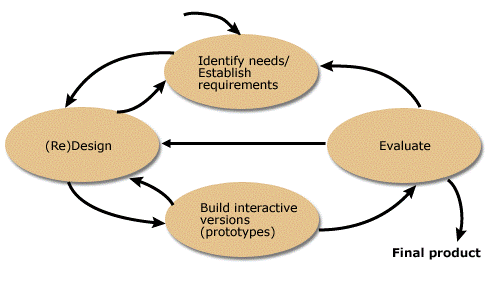
\includegraphics[scale=.8]{images/interatcion-design.png}
  \caption[Interaction design process]{Interaction design process \cite{Sharp2011}}
  \label{fig:interaction_design}
\end{figure}

Identifying needs and establishing requirements is the first and most crucial activity of the process. Its objective is to learn and understand the user needs and communicate them to the developer. According to the chaos report \cite{Group1994}, requirements account for more than the 30\% of the project failure factors, they include lack  of user input, incomplete requirements and specifications, or changes in requirements and specifications. Also its interdisciplinary nature, and contradictions between stakeholders add complexity to this part of the process. To guide it in a more accurate and disciplined manner, it is useful to combine different techniques and methodologies, such as questionnaires, interviews, introspection and brainstorming \cite{Coulin2005}. The selected methods were questionnaires and interviews. Interviews allowed to establish a casual conversation with few potential application users, whereas questionnaires allowed to get different points of views of many potential users of the application. 

A support tool for developing alternative designs is the prototype. It is a physical, or digital outline of a screen or task supported by the product. It allows for different purposes: first, as support for the creative process, allowing the designer to print how is the interface expected to look like and how it will support the intended use cases. Second, as a communication tool for the stakeholders, supporting the flow of ideas between the designer and the people involved in the development. And third, as a testing tool, allowing the designer to get measurable feedback of the capabilities of the product. Prototypes were designed and evaluated in different iterations among the project.
\section{Agile methodology}
The development process followed an agile methodology as a good software engineering practice. The benefit of this approach is that more focus is paid to the product than to the management process. This has proven to be a strong advantage when working on constantly-changing and time-constrained projects such as this dissertation project.
The agile manifesto \cite{Martin2002} establishes four values to guide a development process: 
\begin{displayquote}
\begin{itemize}
  \item Individuals and interactions over processes and tools
  \item Working software over comprehensive documentation
  \item Customer collaboration over contract negotiation
  \item Responding to change over following a plan. 
\end{itemize}
\end{displayquote}

Agility moves the interest in software development towards product functionality rather than product documentation. It recognises that much time can be spent on documenting and planning and stimulates smart resource usage instead by working closely with the stakeholders, responding to change and prioritising software components that have direct interaction with the user. This allows the developer to output iterations to the user for evaluating earlier in the development process.

\iffalse
\subsection{Self-management}
Versioning software was used to manage the workflow of the different components of the system, the repositories are available online in a public GitHub repository. Links
\fi
\section{Evaluation}
Considering that a deliverable of my project dissertation is a mobile application that includes technical and design aspects, the evaluation should be qualitative and quantitative. It should be quantitative to collect measurable indicators of how well the user-requirements were met from a software engineering perspective. Also, qualitative to get an insight from an interaction-design perspective to collect thoughts and reflections about the product.

\subsection{Technical evaluation}
A technical evaluation will ensure that the software behaves as expected during deployment. This will be done by inspecting and debugging the code through the entire development process. Code inspections are performed by visually inspecting the program coded statements and allow for the discovery of logic and coding errors in order to spend less time and effort debugging \cite{Myers2011}. The coding errors that are not discovered on the inspection process will show up when executing the program and may be fixed by debugging. The debugging process finds and corrects suspected errors within the program effortlessly by the use of debugging tools integrated into modern development editors. Once the software development stage has been exhausted, automated tests will be used to discover errors that may still be present.

\subsection{Evaluation with users}
Although designing for usability is the priority, users during the testing phase are expected to use computers and smartphones confidently. Otherwise, tasks within the system will not be carried out independently and may skew gathered results. 

Of particular interest is the level of satisfaction of the app with the user. This will involve collecting measurable indicators of how well the non-functional and functional requirements were met by the application. In other words, to assess how well people can understand and use a product or prototype.

\quotes{This method is accomplished by identifying representative users, representative tasks, and developing a procedure for capturing the problems that users have in trying to apply a particular software product in accomplishing these tasks.} \cite{Scholtz2003} The advantage is the involvement of the user; however, the test attendants should be a representative group of the potential final users of the product. The selected tasks should aim to be as realistic as possible because \quotes{results are based on actually seeing what aspects of the user interface cause problems for representative users}. \cite{Scholtz2003}

\subsection{Design critique}
The objective of including this method is to gather impressions and thoughts about the system and foster an open space to discover what the development of future releases should aim for. According to Blevis et al. \cite{Blevis2007} it allows for understanding the development from the perspective of the user. In this case it will try to understand how the users would include such a development in their daily lives. For instance, if they would be willing to use it on a regular basis because it is attractive and fun to use, or just because they feel it would benefit their health. All of this feedback would give a deeper understanding of the flaws and strengths of the system.

\iffalse
\quotes{Process of discourse on many levels of the nature and effects of an ultimate particular design}. \quotes{Comment on the qualities of an ultimate particular from an holistic perspective, including reason, ethics, and aesthetics as well as minute details of form and external effects on culture}.\cite{Blevis2007}
\fi


\iffalse\section{Out of Scope Issues}\fi

\bibliography{mendeley}
\bibliographystyle{IEEEtranN}
\end{document}
